\documentclass[a4paper]{article}

%================================================================================================================================
%
% Packages
%
%================================================================================================================================

\usepackage[T1]{fontenc} 	% pour caractères accentués
\usepackage[utf8]{inputenc}  % encodage utf8
\usepackage[french]{babel}	% langue : français
\usepackage{fourier}			% caractères plus lisibles
\usepackage[dvipsnames]{xcolor} % couleurs
\usepackage{fancyhdr}		% réglage header footer
\usepackage{needspace}		% empêcher sauts de page mal placés
\usepackage{graphicx}		% pour inclure des graphiques
\usepackage{enumitem,cprotect}		% personnalise les listes d'items (nécessaire pour ol, al ...)
\usepackage{hyperref}		% Liens hypertexte
\usepackage{pstricks,pst-all,pst-node,pstricks-add,pst-math,pst-plot,pst-tree,pst-eucl} % pstricks
\usepackage[a4paper,includeheadfoot,top=2cm,left=3cm, bottom=2cm,right=3cm]{geometry} % marges etc.
\usepackage{comment}			% commentaires multilignes
\usepackage{amsmath,environ} % maths (matrices, etc.)
\usepackage{amssymb,makeidx}
\usepackage{bm}				% bold maths
\usepackage{tabularx}		% tableaux
\usepackage{colortbl}		% tableaux en couleur
\usepackage{fontawesome}		% Fontawesome
\usepackage{environ}			% environment with command
\usepackage{fp}				% calculs pour ps-tricks
\usepackage{multido}			% pour ps tricks
\usepackage[np]{numprint}	% formattage nombre
\usepackage{tikz,tkz-tab} 			% package principal TikZ
\usepackage{pgfplots}   % axes
\usepackage{mathrsfs}    % cursives
\usepackage{calc}			% calcul taille boites
\usepackage[scaled=0.875]{helvet} % font sans serif
\usepackage{svg} % svg
\usepackage{scrextend} % local margin
\usepackage{scratch} %scratch
\usepackage{multicol} % colonnes
%\usepackage{infix-RPN,pst-func} % formule en notation polanaise inversée
\usepackage{listings}

%================================================================================================================================
%
% Réglages de base
%
%================================================================================================================================

\lstset{
language=Python,   % R code
literate=
{á}{{\'a}}1
{à}{{\`a}}1
{ã}{{\~a}}1
{é}{{\'e}}1
{è}{{\`e}}1
{ê}{{\^e}}1
{í}{{\'i}}1
{ó}{{\'o}}1
{õ}{{\~o}}1
{ú}{{\'u}}1
{ü}{{\"u}}1
{ç}{{\c{c}}}1
{~}{{ }}1
}


\definecolor{codegreen}{rgb}{0,0.6,0}
\definecolor{codegray}{rgb}{0.5,0.5,0.5}
\definecolor{codepurple}{rgb}{0.58,0,0.82}
\definecolor{backcolour}{rgb}{0.95,0.95,0.92}

\lstdefinestyle{mystyle}{
    backgroundcolor=\color{backcolour},   
    commentstyle=\color{codegreen},
    keywordstyle=\color{magenta},
    numberstyle=\tiny\color{codegray},
    stringstyle=\color{codepurple},
    basicstyle=\ttfamily\footnotesize,
    breakatwhitespace=false,         
    breaklines=true,                 
    captionpos=b,                    
    keepspaces=true,                 
    numbers=left,                    
xleftmargin=2em,
framexleftmargin=2em,            
    showspaces=false,                
    showstringspaces=false,
    showtabs=false,                  
    tabsize=2,
    upquote=true
}

\lstset{style=mystyle}


\lstset{style=mystyle}
\newcommand{\imgdir}{C:/laragon/www/newmc/assets/imgsvg/}
\newcommand{\imgsvgdir}{C:/laragon/www/newmc/assets/imgsvg/}

\definecolor{mcgris}{RGB}{220, 220, 220}% ancien~; pour compatibilité
\definecolor{mcbleu}{RGB}{52, 152, 219}
\definecolor{mcvert}{RGB}{125, 194, 70}
\definecolor{mcmauve}{RGB}{154, 0, 215}
\definecolor{mcorange}{RGB}{255, 96, 0}
\definecolor{mcturquoise}{RGB}{0, 153, 153}
\definecolor{mcrouge}{RGB}{255, 0, 0}
\definecolor{mclightvert}{RGB}{205, 234, 190}

\definecolor{gris}{RGB}{220, 220, 220}
\definecolor{bleu}{RGB}{52, 152, 219}
\definecolor{vert}{RGB}{125, 194, 70}
\definecolor{mauve}{RGB}{154, 0, 215}
\definecolor{orange}{RGB}{255, 96, 0}
\definecolor{turquoise}{RGB}{0, 153, 153}
\definecolor{rouge}{RGB}{255, 0, 0}
\definecolor{lightvert}{RGB}{205, 234, 190}
\setitemize[0]{label=\color{lightvert}  $\bullet$}

\pagestyle{fancy}
\renewcommand{\headrulewidth}{0.2pt}
\fancyhead[L]{maths-cours.fr}
\fancyhead[R]{\thepage}
\renewcommand{\footrulewidth}{0.2pt}
\fancyfoot[C]{}

\newcolumntype{C}{>{\centering\arraybackslash}X}
\newcolumntype{s}{>{\hsize=.35\hsize\arraybackslash}X}

\setlength{\parindent}{0pt}		 
\setlength{\parskip}{3mm}
\setlength{\headheight}{1cm}

\def\ebook{ebook}
\def\book{book}
\def\web{web}
\def\type{web}

\newcommand{\vect}[1]{\overrightarrow{\,\mathstrut#1\,}}

\def\Oij{$\left(\text{O}~;~\vect{\imath},~\vect{\jmath}\right)$}
\def\Oijk{$\left(\text{O}~;~\vect{\imath},~\vect{\jmath},~\vect{k}\right)$}
\def\Ouv{$\left(\text{O}~;~\vect{u},~\vect{v}\right)$}

\hypersetup{breaklinks=true, colorlinks = true, linkcolor = OliveGreen, urlcolor = OliveGreen, citecolor = OliveGreen, pdfauthor={Didier BONNEL - https://www.maths-cours.fr} } % supprime les bordures autour des liens

\renewcommand{\arg}[0]{\text{arg}}

\everymath{\displaystyle}

%================================================================================================================================
%
% Macros - Commandes
%
%================================================================================================================================

\newcommand\meta[2]{    			% Utilisé pour créer le post HTML.
	\def\titre{titre}
	\def\url{url}
	\def\arg{#1}
	\ifx\titre\arg
		\newcommand\maintitle{#2}
		\fancyhead[L]{#2}
		{\Large\sffamily \MakeUppercase{#2}}
		\vspace{1mm}\textcolor{mcvert}{\hrule}
	\fi 
	\ifx\url\arg
		\fancyfoot[L]{\href{https://www.maths-cours.fr#2}{\black \footnotesize{https://www.maths-cours.fr#2}}}
	\fi 
}


\newcommand\TitreC[1]{    		% Titre centré
     \needspace{3\baselineskip}
     \begin{center}\textbf{#1}\end{center}
}

\newcommand\newpar{    		% paragraphe
     \par
}

\newcommand\nosp {    		% commande vide (pas d'espace)
}
\newcommand{\id}[1]{} %ignore

\newcommand\boite[2]{				% Boite simple sans titre
	\vspace{5mm}
	\setlength{\fboxrule}{0.2mm}
	\setlength{\fboxsep}{5mm}	
	\fcolorbox{#1}{#1!3}{\makebox[\linewidth-2\fboxrule-2\fboxsep]{
  		\begin{minipage}[t]{\linewidth-2\fboxrule-4\fboxsep}\setlength{\parskip}{3mm}
  			 #2
  		\end{minipage}
	}}
	\vspace{5mm}
}

\newcommand\CBox[4]{				% Boites
	\vspace{5mm}
	\setlength{\fboxrule}{0.2mm}
	\setlength{\fboxsep}{5mm}
	
	\fcolorbox{#1}{#1!3}{\makebox[\linewidth-2\fboxrule-2\fboxsep]{
		\begin{minipage}[t]{1cm}\setlength{\parskip}{3mm}
	  		\textcolor{#1}{\LARGE{#2}}    
 	 	\end{minipage}  
  		\begin{minipage}[t]{\linewidth-2\fboxrule-4\fboxsep}\setlength{\parskip}{3mm}
			\raisebox{1.2mm}{\normalsize\sffamily{\textcolor{#1}{#3}}}						
  			 #4
  		\end{minipage}
	}}
	\vspace{5mm}
}

\newcommand\cadre[3]{				% Boites convertible html
	\par
	\vspace{2mm}
	\setlength{\fboxrule}{0.1mm}
	\setlength{\fboxsep}{5mm}
	\fcolorbox{#1}{white}{\makebox[\linewidth-2\fboxrule-2\fboxsep]{
  		\begin{minipage}[t]{\linewidth-2\fboxrule-4\fboxsep}\setlength{\parskip}{3mm}
			\raisebox{-2.5mm}{\sffamily \small{\textcolor{#1}{\MakeUppercase{#2}}}}		
			\par		
  			 #3
 	 		\end{minipage}
	}}
		\vspace{2mm}
	\par
}

\newcommand\bloc[3]{				% Boites convertible html sans bordure
     \needspace{2\baselineskip}
     {\sffamily \small{\textcolor{#1}{\MakeUppercase{#2}}}}    
		\par		
  			 #3
		\par
}

\newcommand\CHelp[1]{
     \CBox{Plum}{\faInfoCircle}{À RETENIR}{#1}
}

\newcommand\CUp[1]{
     \CBox{NavyBlue}{\faThumbsOUp}{EN PRATIQUE}{#1}
}

\newcommand\CInfo[1]{
     \CBox{Sepia}{\faArrowCircleRight}{REMARQUE}{#1}
}

\newcommand\CRedac[1]{
     \CBox{PineGreen}{\faEdit}{BIEN R\'EDIGER}{#1}
}

\newcommand\CError[1]{
     \CBox{Red}{\faExclamationTriangle}{ATTENTION}{#1}
}

\newcommand\TitreExo[2]{
\needspace{4\baselineskip}
 {\sffamily\large EXERCICE #1\ (\emph{#2 points})}
\vspace{5mm}
}

\newcommand\img[2]{
          \includegraphics[width=#2\paperwidth]{\imgdir#1}
}

\newcommand\imgsvg[2]{
       \begin{center}   \includegraphics[width=#2\paperwidth]{\imgsvgdir#1} \end{center}
}


\newcommand\Lien[2]{
     \href{#1}{#2 \tiny \faExternalLink}
}
\newcommand\mcLien[2]{
     \href{https~://www.maths-cours.fr/#1}{#2 \tiny \faExternalLink}
}

\newcommand{\euro}{\eurologo{}}

%================================================================================================================================
%
% Macros - Environement
%
%================================================================================================================================

\newenvironment{tex}{ %
}
{%
}

\newenvironment{indente}{ %
	\setlength\parindent{10mm}
}

{
	\setlength\parindent{0mm}
}

\newenvironment{corrige}{%
     \needspace{3\baselineskip}
     \medskip
     \textbf{\textsc{Corrigé}}
     \medskip
}
{
}

\newenvironment{extern}{%
     \begin{center}
     }
     {
     \end{center}
}

\NewEnviron{code}{%
	\par
     \boite{gray}{\texttt{%
     \BODY
     }}
     \par
}

\newenvironment{vbloc}{% boite sans cadre empeche saut de page
     \begin{minipage}[t]{\linewidth}
     }
     {
     \end{minipage}
}
\NewEnviron{h2}{%
    \needspace{3\baselineskip}
    \vspace{0.6cm}
	\noindent \MakeUppercase{\sffamily \large \BODY}
	\vspace{1mm}\textcolor{mcgris}{\hrule}\vspace{0.4cm}
	\par
}{}

\NewEnviron{h3}{%
    \needspace{3\baselineskip}
	\vspace{5mm}
	\textsc{\BODY}
	\par
}

\NewEnviron{margeneg}{ %
\begin{addmargin}[-1cm]{0cm}
\BODY
\end{addmargin}
}

\NewEnviron{html}{%
}

\begin{document}
\meta{url}{/exercices/graphes-bac-blanc-es-sujet-1-maths-cours-2018-spe/}
\meta{pid}{10428}
\meta{titre}{Graphes - Bac blanc ES Sujet 1 - Maths-cours 2018 (spé)}
\meta{type}{exercices}
%
\begin{h2}Exercice 4 (5 points)\end{h2}
\par
\textbf{Candidats ayant suivi l'enseignement de spécialité}
\par
Un appartement comporte 6 pièces notées A, B, C, D, E et F.
\par
Le plan ci-après présente la disposition des pièces ainsi que les portes de communication entre ces pièces.
\par
\begin{center}
     \begin{extern}%width="500" alt="Plan et graphes"
          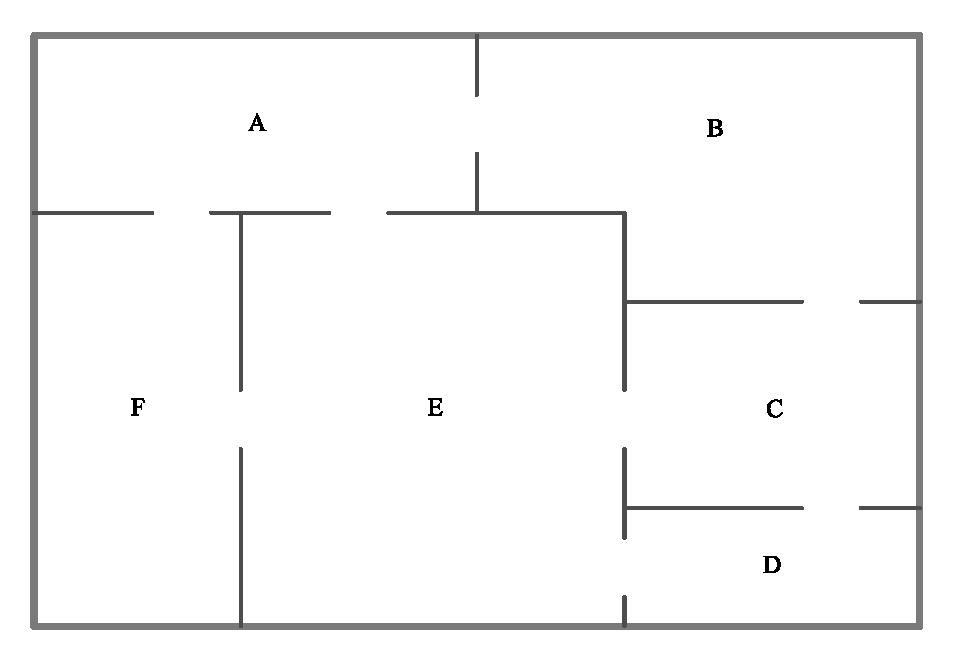
\includegraphics[width=0.9\textwidth]{images/BBESL-spe-1-1}% gbb 1 unite=1cm
     \end{extern}
\end{center}
\par
Par exemple, il y a une porte de communication entre les pièces A et B mais il n'y en a pas entre les pièces B et E.
\par
La porte donnant accès à l'appartement est sans importance dans le cadre de l'exercice et n'a pas été représentée.
\par
\textit{Toutes les réponses aux questions posées devront être justifiées.}
\par
\begin{enumerate}
     \item %1

     \begin{enumerate}[label=\alph*.]
          \item %1a
          Traduire la situation à l'aide d'un graphe (G) dont les sommets représentent les pièces et dont les arêtes représentent les portes de communication.
          \item %1b
          Le graphe (G) est-il connexe ? complet ?
     \end{enumerate}
     \par
     \item %2
     \begin{enumerate}[label=\alph*.]
          \item %2a
          Est-il possible de parcourir l'appartement en empruntant chaque porte une fois et une seule ?\\
          Si oui, donner un exemple d'un tel chemin.
          \item %2b
          Est-il possible de parcourir l'appartement en empruntant chaque porte une fois et une seule et \textit{en partant et en arrivant dans la même pièce} ?\\
          Si oui, donner un exemple d'un tel chemin.
     \end{enumerate}
    
     \item %3
     Déterminer la matrice de transition $M$ associée au graphe précédent en prenant les sommets par ordre alphabétique.
   
     \item %4
    
     \`A l'aide d'une calculatrice on trouve~:
     \[ M^3 = \begin{pmatrix}
          2 &5 &2 &3 &7 &4 \\
          5 &0 &5 &2 &2 &2 \\
          2 &5 &2 &4 &7 &3 \\
          3 &2 &4 &2 &5 &2 \\
          7 &2 &7 &5 &4 &5\\
     4 &2 &3 &2 &5 &2  \end{pmatrix} \]
     \begin{enumerate}[label=\alph*.]
          \item %4a
          \par
          Combien existe-t-il de chemins permettant d'aller de la pièce A à la pièce D en empruntant exactement trois portes ?\\
          Donner la liste de ces chemins.

          \item %4b

          Est-il toujours possible de relier deux pièces différentes en empruntant exactement trois portes ?
          \par
     \end{enumerate}
     \par
     \item %5
    
     \begin{enumerate}[label=\alph*.]
          \item %5a
         
          Montrer qu'il existe au moins un sous-graphe \textit{complet} de (G) d'ordre 3.
          \par
          \item %5b
          
          Le propriétaire souhaite repeindre l'appartement en respectant les règles suivantes~:
          \par
          \begin{itemize}
               \item %
               chaque pièce sera repeinte avec une couleur unique~;
               \item %
               deux pièces adjacentes, c'est à dire reliées par une porte, seront repeintes avec des couleurs différentes.
          \end{itemize}
          \par
          Pourra-t-il réaliser ces objectifs en utilisant seulement trois couleurs ?
     \end{enumerate}
\end{enumerate}
\begin{corrige}
     \begin{enumerate}
          \item %1
          \par
          \begin{enumerate}[label=\alph*.]
               \item %1a
               On place d'abord les sommets A, B, C, D, E et F qui représentent les pièces et on relie, par des arêtes, les pièces qui communiquent~: A-B, A-E, A-F, B-C, C-D, C-E, D-E, E-F.
               \par
               \begin{center}
                    \begin{extern}%width="2_0" alt="Graphe communications entre pièces"
                         \psset{unit=0.7cm}
                         \begin{pspicture}(10,7)
                              \rput(2,6){\circlenode{A}{A}}
                              \rput(6,6){\circlenode{B}{B}}
                              \rput(9,4){\circlenode{C}{C}}
                              \rput(8,1){\circlenode{D}{D}}
                              \rput(5,4){\circlenode{E}{E}}
                              \rput(1,2){\circlenode{F}{F}}
                              \ncline{A}{B}
                              \ncline{A}{E}
                              \ncline{B}{C}
                              \ncline{C}{D}
                              \ncline{D}{E}
                              \ncline{A}{F}
                              \ncline{E}{F}
                              \ncline{E}{C}
                         \end{pspicture}
                    \end{extern}
               \end{center}
               \par
               \item %1b
               Le graphe est \textbf{connexe}. En effet, un graphe est connexe si deux sommets quelconques peuvent être reliés par une chaîne ce qui est le cas ici.
               \par
               Le graphe \textbf{n'est pas complet}. Un graphe non orienté est complet si et seulement si tous ses sommets sont reliés par une arête. Ce n'est pas le cas ici pour A et C par exemple.
               \cadre{rouge}{À retenir}{
                    Un graphe est \textbf{complet} si et seulement si tous ses sommets sont deux à deux adjacents (c'est à dire reliés par une arête).
                    \par
                    Un graphe est \textbf{connexe} si et seulement si deux sommets quelconques peuvent être reliés par une chaîne (intuitivement cela signifie que le graphe est en \og un seul morceau \fg{}).
               }
          \end{enumerate}
          \par
          \item %2
          \par
          \begin{enumerate}[label=\alph*.]
               \item %2a
               On recherche s'il existe une \textbf{chaîne eulérienne}, c'est à dire une chaîne qui contient une fois et une seule chacune des arêtes du graphe.
               \par
               D'après le théorème d'Euler, un graphe connexe contient une chaîne eulérienne si et seulement s'il possède \textbf{0 ou 2 sommets de degré impair}.
               \par
               Le degré de chacun des sommets est donné par le tableau ci-après~:
               \par
               \begin{center}
                    \begin{tabular}{|l|c|c|c|c|c|c|c|c|}%class="compact"
                         \hline
                         Sommet & A & B & C & D & E & F  \\
                         \hline
                         Degré & 3 & 2 & 3 & 2 & 4 & 2 \\
                         \hline
                    \end{tabular}
               \end{center}
               \par
               Le graphe (G) possède \textbf{deux} sommets de degré impair~: A et C.
               \par
               Il est donc \textbf{possible} de parcourir l'appartement en empruntant chacune des 8 portes une fois et une seule, par exemple en suivant le trajet~: A-B-C-D-E-F-A-E-C.
               \par
               \cadre{rouge}{À retenir}{
                    Une \textbf{chaîne eulérienne} est une chaîne qui contient une fois et une seule chacune des arêtes du graphe.
                    \par
                    Trouver un chemin qui emprunte chaque arête une fois et une seule revient à trouver une chaîne eulérienne.
                    \par
                    Un graphe connexe admet une \textbf{chaîne eulérienne} si et seulement s'il possède \textbf{0 ou 2 sommet(s) de degré impair}.
               }
               \par
               \item %2b
               Dans cette question, on recherche l'existence d'un \textbf{cycle eulérien} (un cycle est une chaîne fermée).
               \par
               Or, d'après le théorème d'Euler, un graphe connexe contient un cycle eulérien si et seulement s'il ne possède \textbf{aucun sommet de degré impair}.
               \par
               Ici, A et C sont de degré impair. Toute chaîne eulérienne aura pour extrémités A et C et ne sera donc pas un cycle.
               \par
               Par conséquent, \textbf{il n'est pas possible} de parcourir l'appartement en empruntant chaque porte une fois et une seule et en partant et en arrivant dans la même pièce.
               \par
               \cadre{rouge}{À retenir}{
                    Un \textbf{cycle eulérien} est une chaîne \textbf{fermée} qui contient une fois et une seule chacune des arêtes du graphe.
                    \par
                    Trouver un chemin qui emprunte chaque arête une fois et une seule et dont \textit{les sommets de départ et d'arrivée sont identiques}  revient à trouver un cycle eulérien.
                    \par
                    Un graphe connexe admet un \textbf{cycle eulérien} si et seulement s'il ne possède \textbf{aucun sommet de degré impair}.
               }
               \par
          \end{enumerate}
          \par
          \item %3
          Numérotons les pièces A: 1, B: 2, C: 3, D: 4, E: 5, F: 6.\\
          La matrice de transition $M$ associée au graphe précédent s'obtient en plaçant à la $i$-ième ligne et à la $j$-ième colonne~:
          \begin{itemize}
               \item %
               un \og 1 \fg{} si les pièces numérotées $i$ et $j$ sont reliés par une arête~;
               \item %
               un \og 0 \fg{} sinon.
          \end{itemize}
          \par
          On obtient alors la matrice~:
          \par
          \[ M = \begin{pmatrix}
               0 &1 &0 &0 &1 &1 \\
               1 &0 &1 &0 &0 &0 \\
               0 &1 &0 &1 &1 &0 \\
               0 &0 &1 &0 &1 &0 \\
               1 &0 &1 &1 &0 &1\\
          1 &0 &0 &0 &1 &0  \end{pmatrix} \]
          \par
          \item %4
          \par
          \begin{enumerate}[label=\alph*.]
               \item %4a
               \par
               Le coefficient de $M^3$ situé à la $i$-ième ligne et à la $j$-ième colonne indique le nombre de chemins de trois arêtes menant du sommet numéro $i$ au sommet numéro $j$.
               \par
               Ici, le coefficient situé à la première ligne et à la quatrième colonne est 3. Il y a donc 3 chemins permettant d'aller de la pièce A à la pièce D en empruntant exactement trois portes.
               \par
               \`A l'aide du graphe, on trouve les chemins~: A-B-C-D, A-E-C-D et A-F-E-D.
               \par
               \cadre{rouge}{À retenir}{
                    Le coefficient de la matrice $M^n$ situé à la $i$-ième ligne et à la $j$-ième colonne correspond au nombre de chemins \textbf{de longueur} $\bm{n}$ menant du sommet numéro $i$ au sommet numéro $j$.
               }
               \par
               \item %4b
               \par
               La matrice $M^3$ comporte un unique coefficient nul situé en ligne 2 et en colonne 2. Cela signifie qu'il n'est pas possible de partir de la pièce B pour revenir à la pièce B en empruntant exactement 3 portes mais que, mis à part ce cas, il est toujours possible de joindre deux pièces en empruntant exactement 3 portes.
               \par
               Comme l'énoncé précise deux pièces \textbf{différentes}, il est effectivement \textbf{toujours possible} de joindre deux pièces différentes en empruntant exactement trois portes.
          \end{enumerate}
          \par
          \item %5
          \par
          \begin{enumerate}[label=\alph*.]
               \item %5a
               Considérons le sous-graphe constitué des sommets A, E et F. Chacun de ces trois sommets est relié aux deux autres, donc \textbf{ce sous-graphe est complet}. Le sous-graphe constitué de C, E et D est lui-aussi complet.
               \par
               \item %5b
               \par
               Il est possible de repeindre les pièces en respectant les consignes de l'énoncé et avec seulement trois couleurs.
               \par
               Le sous-graphe A, E et F étant complet, il faudra nécessairement trois couleurs différentes pour peindre ces trois pièces.\\
               Il en est de même pour les pièces C, E et D.
               \par
               En respectant ces contraintes, il est facile de trouver une solution au problème posé~; par exemple (mais il y a d'autres solutions ...)~:
               \par
               Couleur 1~: E, B\\
               Couleur 2~: A, C\\
               Couleur 3~: F, D.\\
               \par
          \end{enumerate}
     \end{enumerate}
\end{corrige}

\end{document}